\documentclass[11pt,a4paper]{article}
\usepackage[margin=18mm]{geometry}
\usepackage{amsmath,amssymb,mathtools}
\usepackage{booktabs,array,enumitem}
\usepackage[dvipsnames]{xcolor}
\usepackage{listings}
\usepackage{tikz}
\usetikzlibrary{arrows.meta,positioning}
\usepackage[most]{tcolorbox}
\usepackage{hyperref}
\hypersetup{colorlinks=true,urlcolor=MidnightBlue,linkcolor=MidnightBlue}
\setlength{\parindent}{0pt}
\setlength{\parskip}{4pt}
\newcommand{\course}{Computational Methods in Physics}
\newtcolorbox{keybox}{colback=RoyalBlue!5,colframe=RoyalBlue!65!black,boxrule=.7pt,arc=2mm}
\newtcolorbox{checkbox}{colback=ForestGreen!5,colframe=ForestGreen!55!black,boxrule=.7pt,arc=2mm}
\newtcolorbox{aibox}{colback=BurntOrange!7,colframe=BurntOrange!80!black,boxrule=.7pt,arc=2mm}
\lstdefinestyle{matlabstyle}{
  language=Matlab,
  basicstyle=\ttfamily\footnotesize,
  keywordstyle=\color{RoyalBlue!75!black},
  commentstyle=\color{ForestGreen!55!black},
  stringstyle=\color{BurntOrange!80!black},
  numbers=left,
  numberstyle=\scriptsize\color{black!50},
  numbersep=5pt,
  frame=single,
  rulecolor=\color{RoyalBlue!25},
  backgroundcolor=\color{RoyalBlue!3},
  showstringspaces=false,
  columns=fullflexible,
  keepspaces=true,
  breaklines=true
}
\begin{document}

{\large\textsc{\course}}\\[-2pt]
{\small Learning Note \textbar\ Week 1}\par\vspace{4pt}
{\LARGE\bfseries From a Physics Model to a Computational Experiment}\par\vspace{3pt}
\textit{A numerical result is useful only when its model, units, assumptions, and checks are visible.}

\begin{keybox}
\textbf{Physical question.} A radioactive sample has a half-life of $6.0\,\mathrm{h}$. How can we simulate its decay over one day, and how small must the time step be before we trust the result?
\end{keybox}

\section*{Learning outcomes}
By the end of this week, you should be able to:
\begin{enumerate}[nosep,leftmargin=5mm]
  \item turn a physical question into variables, assumptions, equations, and a numerical procedure;
  \item check dimensions and limiting cases before running a model;
  \item implement the idea of time stepping in MATLAB and plot a result with meaningful axes and units;
  \item compare a numerical result with a reference solution and explain the effect of the time step; and
  \item make a computational experiment reproducible.
\end{enumerate}

\section*{How to use this note}
Read the physical question first, make a prediction, and only then run the MATLAB experiment. The purpose is not to memorise a command sequence; it is to make the model, numerical method, and validation evidence visible.

\begin{keybox}
\textbf{Week 1 bridge.} We use the radioactive-decay problem to practise the minimum MATLAB workflow: name the quantities, write a script, store values in arrays, repeat a time-step rule, plot the result, and test whether the answer deserves trust.
\end{keybox}

\section*{1. The computational-physics cycle}
Computation is not a replacement for physics. It is a controlled experiment performed on a mathematical model.

\begin{center}
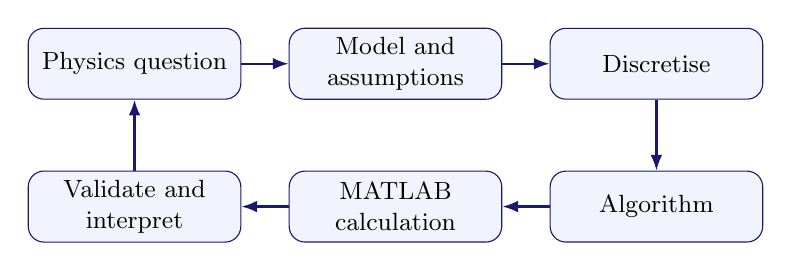
\begin{tikzpicture}[node distance=9mm and 6mm,every node/.style={font=\small,align=center},box/.style={draw=MidnightBlue,rounded corners=2mm,fill=RoyalBlue!7,minimum width=27mm,minimum height=9mm},arrow/.style={-{Latex[length=2mm]},thick,MidnightBlue}]
\node[box] (q) {Physics question};
\node[box,right=of q] (m) {Model and\\assumptions};
\node[box,right=of m] (d) {Discretise};
\node[box,below=of d] (a) {Algorithm};
\node[box,left=of a] (c) {MATLAB\\calculation};
\node[box,left=of c] (v) {Validate and\\interpret};
\draw[arrow] (q)--(m); \draw[arrow] (m)--(d); \draw[arrow] (d)--(a);
\draw[arrow] (a)--(c); \draw[arrow] (c)--(v); \draw[arrow] (v)--(q);
\end{tikzpicture}
\end{center}

At every stage, write down what you know and what you are approximating. A graph alone is not evidence that a simulation is correct.

\section*{2. MATLAB essentials for this experiment}
MATLAB provides several views of the same computational experiment:
\begin{itemize}[nosep,leftmargin=5mm]
  \item the \textbf{Command Window} is useful for trying one expression;
  \item the \textbf{Editor/Live Editor} stores a repeatable plain-text \texttt{.m} Live Script with text, code, and output;
  \item the \textbf{Workspace} shows variables currently in memory; and
  \item the \textbf{Current Folder} identifies the files MATLAB can run without an explicit path.
\end{itemize}

Use meaningful names and make units visible in the name or in a nearby comment. For this week, the essential MATLAB pattern is:
\begin{center}
\small
\begin{tabular}{>{\raggedright\arraybackslash}p{.27\linewidth}p{.61\linewidth}}
\toprule
\textbf{MATLAB idea} & \textbf{Example and purpose}\\ \midrule
Assignment & \texttt{radius\_m = 0.02;} stores a value in a named variable.\\
Arithmetic & \texttt{area\_m2 = pi*radius\_m\string^2;} evaluates an expression.\\
Function & \texttt{lambda\_per\_h = log(2)/T\_half\_h;} calls a built-in function.\\
Comment & \texttt{\% half-life is measured in hours} records a choice for a reader.\\
Fresh run & Open the plain-text \texttt{.m} Live Script in a fresh MATLAB session so old Workspace values cannot hide a mistake.\\ \bottomrule
\end{tabular}
\end{center}

\textbf{Onramp diagnostic bridge: arrays become physical evidence.} The practical transfers the same reasoning chain to Newton's cooling model,
\begin{equation}
  T(t)=T_{\mathrm{env}}+\left(T_0-T_{\mathrm{env}}\right)e^{-kt}.
\end{equation}
With $T_0=80\,^{\circ}\mathrm{C}$, $T_{\mathrm{env}}=22\,^{\circ}\mathrm{C}$, and $k=0.08\,\mathrm{min}^{-1}$, students build a time array, evaluate the model element by element, and locate the first stored time within $1\,^{\circ}\mathrm{C}$ of the room:
\begin{lstlisting}[style=matlabstyle]
t_min = 0:2:60;
T_C = Tenv_C + (T0_C-Tenv_C).*exp(-k_per_min.*t_min);
withinTolerance = abs(T_C-Tenv_C) <= 1;
firstIndex = find(withinTolerance,1,'first');
firstStoredTime_min = t_min(firstIndex)
\end{lstlisting}
The first stored threshold time is $52\,\mathrm{min}$ on this grid. The exact continuous crossing is earlier, so the activity also exposes an important distinction between a physical model and the resolution at which it is sampled. The practical diagnoses prerequisite array, element-wise-operation, indexing, plotting, logic, and validation skills; it does not reteach MATLAB as an end in itself.

\section*{3. Worked physical model: radioactive decay}
Let $N(t)$ be the number of undecayed nuclei. For a closed sample with a constant decay constant $\lambda$,
\begin{equation}
  \frac{dN}{dt}=-\lambda N, \qquad N(0)=N_0.
\end{equation}
The model says that each nucleus has the same probability of decaying per unit time. It ignores, for example, a changing decay constant or nuclei entering or leaving the sample.

The half-life $T_{1/2}$ and decay constant are related by
\begin{equation}
  \lambda = \frac{\ln 2}{T_{1/2}}.
\end{equation}
For $T_{1/2}=6.0\,\mathrm{h}$, $\lambda=0.1155\,\mathrm{h}^{-1}$. Notice the units: $\lambda t$ must be dimensionless.

\textbf{Parameter map.} The physics symbols become MATLAB variables without using Greek letters in the variable names:
\begin{center}
\small
\begin{tabular}{>{\raggedright\arraybackslash}p{.22\linewidth}p{.29\linewidth}p{.34\linewidth}}
\toprule
\textbf{Physics} & \textbf{MATLAB name} & \textbf{Meaning and unit}\\ \midrule
$N_0$ & \texttt{N0} & initial population, nuclei\\
$T_{1/2}$ & \texttt{T\_half\_h} & half-life, hours\\
$\lambda$ & \texttt{lambda\_per\_h} & decay constant, $\mathrm{h}^{-1}$\\
$t_{\max}$ & \texttt{tMax\_h} & final simulated time, hours\\
$\Delta t$ & \texttt{dt\_h} & numerical step size, hours\\ \bottomrule
\end{tabular}
\end{center}

\begin{checkbox}
\textbf{Before computing, predict.}
\begin{itemize}[nosep,leftmargin=5mm]
  \item If $\lambda\to0$, what should happen to $N(t)$?
  \item At $t=6.0\,\mathrm{h}$, what fraction of $N_0$ should remain?
  \item Can a physically meaningful calculation return $N<0$?
\end{itemize}
\end{checkbox}

\section*{4. From differential equation to time-step rule}
Choose equally spaced times $t_n=n\Delta t$. Approximate the derivative with a forward difference:
\begin{equation}
  \frac{N_{n+1}-N_n}{\Delta t}\approx-\lambda N_n.
\end{equation}
Rearranging gives the \textbf{forward Euler} update:
\begin{equation}
  N_{n+1}=N_n\left(1-\lambda\Delta t\right).
\end{equation}
This equation is not the exact physics; it is an approximation to the model. It becomes more accurate as $\Delta t$ decreases, but uses more computational steps.

\textbf{Algorithm.}
\begin{enumerate}[nosep,leftmargin=6mm]
  \item Choose $N_0$, $T_{1/2}$, a final time $t_{\max}$, and $\Delta t$.
  \item Compute $\lambda=\ln2/T_{1/2}$ and create a time array.
  \item Set the first value, $N_1=N_0$.
  \item Apply the Euler update from one time index to the next.
  \item Plot $N/N_0$ against $t$ and compare it with a reference.
\end{enumerate}

The following is a minimal, complete script. It deliberately keeps the model visible: the update rule appears as one line inside the loop.
\begin{lstlisting}[style=matlabstyle,caption={A first Euler simulation}]
N0 = 1000;
T_half_h = 6.0;
tMax_h = 24.0;
dt_h = 0.5;
lambda_per_h = log(2)/T_half_h;

t_h = 0:dt_h:tMax_h;
N = zeros(size(t_h));
N(1) = N0;

for n = 1:numel(t_h)-1
    N(n+1) = N(n)*(1 - lambda_per_h*dt_h);
end

N_exact = N0*exp(-lambda_per_h*t_h);
plot(t_h,N/N0,'o-',t_h,N_exact/N0,'k-','LineWidth',1.5)
xlabel('Time, t (h)'); ylabel('Fraction remaining, N/N_0')
legend('Forward Euler','Exact','Location','northeast')
grid on
\end{lstlisting}

Read the script in three layers: parameters and units, storage and initial condition, then the repeated update. The loop is not a new physical law; it is the computer carrying out the discretised rule.

\section*{5. A reference answer and numerical error}
For this model, the analytic solution is available:
\begin{equation}
  N_{\mathrm{exact}}(t)=N_0e^{-\lambda t}.
\end{equation}
Use it as a benchmark, not as a shortcut that makes numerical work unnecessary. A useful final-time relative error is
\begin{equation}
  \varepsilon_{\mathrm{rel}}=\frac{\left|N_{\mathrm{Euler}}(t_{\max})-N_{\mathrm{exact}}(t_{\max})\right|}{N_{\mathrm{exact}}(t_{\max})}.
\end{equation}

Run the same experiment with $\Delta t=1.0\,\mathrm{h}$, $0.5\,\mathrm{h}$, and $0.1\,\mathrm{h}$. The result should approach the reference as the step becomes smaller. A choice with $\lambda\Delta t>1$ is a warning sign: the Euler update can produce a negative $N$, which is unphysical.

For $T_{1/2}=6.0\,\mathrm{h}$ and $t_{\max}=24\,\mathrm{h}$, the exact fraction is $e^{-\lambda t_{\max}}=0.0625$. The following values are useful checkpoints:
\begin{center}
\small
\begin{tabular}{rrrr}
\toprule
$\Delta t$ (h) & $\lambda\Delta t$ & $N_{\mathrm{Euler}}(24\,\mathrm{h})/N_0$ & relative error\\ \midrule
2.0 & 0.2310 & 0.042735 & 31.62\%\\
1.0 & 0.1155 & 0.052536 & 15.94\%\\
0.5 & 0.0578 & 0.057505 & 7.99\%\\
0.1 & 0.0116 & 0.061499 & 1.60\%\\ \bottomrule
\end{tabular}
\end{center}
Smaller $\Delta t$ improves the approximation here, but it also increases the number of computational steps. A good numerical experiment reports both the result and the cost of obtaining it.

\section*{6. What MATLAB is doing}
MATLAB stores the time points and values in arrays. The code should make the model visible rather than hiding it in unexplained commands.

\begin{center}
\begin{tabular}{>{\raggedright\arraybackslash}p{.28\linewidth}p{.62\linewidth}}
\toprule
\textbf{Object} & \textbf{Meaning in this experiment}\\ \midrule
\texttt{t} & vector of times, with one consistent unit\\
\texttt{N} & vector of computed populations; its first element is the initial condition\\
\texttt{dt} & numerical resolution, not a physical parameter of the isotope\\
\texttt{lambda} & decay constant; use a name that does not conflict with MATLAB functions\\
\texttt{plot(t,N/N0)} & visual comparison of a dimensionless fraction against time\\ \bottomrule
\end{tabular}
\end{center}

Use comments to explain choices such as the time unit and the validation test. Do not rely on the current Workspace: a good script should run correctly after a fresh MATLAB restart.

\textbf{Common errors and quick checks.}
\begin{center}
\small
\begin{tabular}{>{\raggedright\arraybackslash}p{.38\linewidth}>{\raggedright\arraybackslash}p{.48\linewidth}}
\toprule
\textbf{Symptom} & \textbf{First check}\\ \midrule
The curve starts below $N_0$ & Did you set \texttt{N(1) = N0}?\\
The first update is missing & Does the loop write \texttt{N(n+1)} rather than overwrite \texttt{N(n)}?\\
Values become negative & Is $\lambda\Delta t>1$? Check the units of $\lambda$ and $\Delta t$.\\
The plot changes between runs & Start a fresh MATLAB session and confirm every input is defined in the Live Script.\\
The graph cannot be interpreted & Add a title, axis labels, units, legend, and a caption.\\ \bottomrule
\end{tabular}
\end{center}

\newpage
\section*{7. Reproducible computational experiments}
A colleague should be able to reproduce your figure using the same file and inputs. Record:
\begin{itemize}[nosep,leftmargin=5mm]
  \item the physical parameters and their units;
  \item the numerical settings, especially $\Delta t$ and $t_{\max}$;
  \item the MATLAB version or toolboxes if they matter;
  \item the validation method and the result of that check; and
  \item a clear figure title, axis labels, units, and caption.
\end{itemize}

\begin{aibox}
\textbf{AI with responsibility.} An AI assistant may help explain an Euler update or suggest MATLAB syntax. It cannot establish that your result is physically valid. If AI materially influences the work, record what was requested, what was accepted, modified, or rejected, why that decision was made, and which independent checks were performed. At minimum, check the units, reproduce a limiting case, compare with $N_{\mathrm{exact}}$, and interpret the result physically.
\end{aibox}

\textbf{Validation checklist.} Before presenting a computational result, confirm each layer:
\begin{center}
\small
\begin{tabular}{>{\raggedright\arraybackslash}p{.23\linewidth}>{\raggedright\arraybackslash}p{.62\linewidth}}
\toprule
\textbf{Layer} & \textbf{Evidence to record}\\ \midrule
Physics & State the question, variables, assumptions, and expected trend.\\
Units & Check that $\lambda$ and $t$ use the same time unit, so $\lambda t$ is dimensionless.\\
Algorithm & Show the update rule and identify the initial condition and index range.\\
Numerics & Compare at least two timesteps and report an error or convergence measure.\\
Communication & Label the figure, include units, and write one sentence interpreting it.\\ \bottomrule
\end{tabular}
\end{center}

\textbf{Experiment record.} Use this compact record when you run the Live Script or present your result:
\begin{center}
\small
\begin{tabular}{>{\raggedright\arraybackslash}p{.27\linewidth}>{\raggedright\arraybackslash}p{.58\linewidth}}
\toprule
\textbf{Item} & \textbf{Record}\\ \midrule
Physical question & What quantity is being predicted?\\
Parameters and units & $N_0=$\rule{18mm}{0.3pt}, $T_{1/2}=$\rule{15mm}{0.3pt}, $t_{\max}=$\rule{15mm}{0.3pt}.\\
Numerical settings & $\Delta t=$\rule{15mm}{0.3pt}; number of steps $=$\rule{15mm}{0.3pt}.\\
Validation evidence & Reference / limiting case / timestep comparison: \rule{35mm}{0.3pt}.\\
Interpretation & My result is / is not adequate because \rule{28mm}{0.3pt}.\\ \bottomrule
\end{tabular}
\end{center}

\section*{8. Guided practice and self-check}
Work through these tasks before looking at the answer hints:
\begin{enumerate}[nosep,leftmargin=6mm]
  \item \textbf{Predict.} What fractions should remain after one, two, and four half-lives? Explain why the answer does not depend on $N_0$.
  \item \textbf{Complete.} Fill in the missing MATLAB update: \texttt{N(n+1) = N(n)*(1 - ... );}. State the unit of the product inside the brackets.
  \item \textbf{Experiment.} Change $T_{1/2}$ to $3.0\,\mathrm{h}$ and compare the exact fraction at 24 hours with the original model. Keep the time unit consistent.
  \item \textbf{Debug.} A classmate's script gives a negative population and an unlabeled figure. Identify two numerical issues and two communication issues.
\end{enumerate}

\begin{checkbox}
\textbf{Exit ticket.} Submit three sentences: (1) the model equation and one assumption, (2) the MATLAB line that advances one time step, and (3) the validation evidence that makes your chosen $\Delta t$ acceptable.
\end{checkbox}

\section*{Glossary}
\begin{center}
\small
\begin{tabular}{>{\raggedright\arraybackslash}p{.24\linewidth}p{.63\linewidth}}
\toprule
\textbf{Term} & \textbf{Meaning in this note}\\ \midrule
Model & Mathematical description of a physical system and its assumptions.\\
State variable & Quantity whose value changes during the simulation, such as $N(t)$.\\
Parameter & Fixed input that defines the model, such as $T_{1/2}$ or $\lambda$.\\
Exact solution & A reference solution obtained without the timestep approximation.\\
Numerical solution & An approximate solution produced by a discrete algorithm.\\
Timestep & The numerical interval $\Delta t$ between successive computed values.\\
Validation & Evidence that the implementation and interpretation agree with a trusted check.\\
Reproducibility & The ability of another person to rerun the same experiment from the recorded inputs and file.\\ \bottomrule
\end{tabular}
\end{center}

\section*{Three takeaways}
\begin{enumerate}[nosep,leftmargin=5mm]
  \item \textbf{A computational result begins with a model and assumptions, not with a MATLAB command.}
  \item \textbf{A time step is part of the numerical method and must be tested.}
  \item \textbf{Validation and interpretation are required parts of a simulation.}
\end{enumerate}

\begin{keybox}
\textbf{Preparation for the practical.} Complete the individual AI-free entry check, then open \texttt{PHY4605\_Week01\_Onramp\_Diagnostic.m} in MATLAB R2025a or later. Record the cooling prediction before using Copilot. Be ready to show the model and units, explain one array operation and one loop update, diagnose a plausible defective solution, and defend the validation evidence.
\end{keybox}
\end{document}
